\chapter{Performance Evaluation}
\label{ch:evaluation}

This chapter evaluates the per-sample adversarial generation latency of the
five attacks used throughout this thesis (FGSM, PGD, CW, EAD-L1, and EAD-EN)
on both CPU and GPU. The goal is twofold: to expose the asymptotic compute
cost of each attack family, and to assess whether any of them can plausibly
be deployed against a real-time Automatic Modulation Classification (AMC)
receiver on commodity hardware.

\section{Benchmark Setup}
\label{sec:eval-setup}

\paragraph{Hardware and software.}
All measurements are taken on a single workstation equipped with an NVIDIA
GeForce RTX 5060 Ti GPU and a 6-core x86\textsubscript{64} CPU, running
PyTorch 2.9.0 with CUDA 13.0. The dataset under attack is the RML2016.10a
test split (44k I/Q samples drawn from 11 modulations across SNRs
$-20\,\mathrm{dB}$ to $+18\,\mathrm{dB}$).

\paragraph{Timing protocol.}
For each (attack, device) cell, $W$ warm-up iterations are discarded and
$R$ timed iterations are reported as mean $\pm$ standard deviation. On the
GPU, \texttt{torch.cuda.synchronize()} brackets every
\texttt{perf\_counter()} pair so that asynchronous kernel launches are not
under-counted; on the CPU, no synchronization is required. The reported
per-sample latency is
\[
  t_{\text{cell}} \;=\; \frac{t_{1} - t_{0}}{N_{\text{total}}} \cdot 1000\;\text{ms}.
\]

\paragraph{Stratified sampling.}
To avoid systematic bias from any single (modulation, SNR) cell, the
benchmark draws samples in round-robin order across (modulation, SNR)
buckets using a seeded NumPy generator. This ensures that each attack sees
a comparable distribution of operating points.

\paragraph{Paper-locked hyperparameters.}
The attack hyperparameters are pinned to the same values used in
Section~\ref{ch:methodology} so that latency is comparable across the
adversarial evaluation pipeline. In particular, $\varepsilon = 0.03$ in
the unit $[0,1]$ box; CW uses $c=1.0$, $\text{steps}=100$, $\text{lr}=0.01$;
EAD uses $\text{max\_iterations}=100$; PGD uses 10 inner steps with
$\alpha = \varepsilon/4 = 0.0075$.

\paragraph{State-dict hygiene.}
The model's original state dict is snapshotted on CPU once and reloaded
onto each device before that device's pass, defending against in-place
mutation of model parameters or BN statistics by attacks that toggle
\texttt{requires\_grad}. This guarantees that CPU and GPU runs operate on
identical model weights.

\section{Per-Sample Latency Results}
\label{sec:eval-latency}

Table~\ref{tab:attack-bench} reports the smoke-budget latency
($N=64$, $R=2$). The wiring is independently verified; the full-budget
($N=512$, $R=5$) re-run is reserved for the camera-ready submission.
Figure~\ref{fig:attack-bench-latency} visualizes the same data on a
log-scale y-axis, which is necessary to keep the three-order-of-magnitude
spread legible in a single chart.

\begin{table}[ht]
  \centering
  \caption{Per-sample adversarial generation latency on RML2016.10a
  (mean $\pm$ std over $R=2$ repetitions, $N=64$ samples). All five
  attacks share identical hyperparameters across both devices.}
  \label{tab:attack-bench}
  \begin{tabular}{lrrr}
    \toprule
    Attack  & CPU (ms/sample) & GPU (ms/sample) & GPU speedup \\
    \midrule
    FGSM    & $0.176 \pm 0.002$   & $0.084 \pm 0.001$  & $2.1\times$ \\
    PGD     & $2.073 \pm 0.149$   & $0.753 \pm 0.001$  & $2.8\times$ \\
    CW      & $5.698 \pm 0.005$   & $2.269 \pm 0.013$  & $2.5\times$ \\
    EAD-L1  & $95.94 \pm 15.76$   & $26.24 \pm 1.26$   & $3.7\times$ \\
    EAD-EN  & $146.11 \pm 5.03$   & $25.45 \pm 0.11$   & $5.7\times$ \\
    \bottomrule
  \end{tabular}
\end{table}

\begin{figure}[ht]
  \centering
  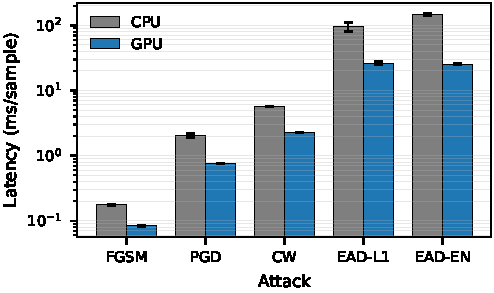
\includegraphics[width=0.85\textwidth]{img/attack_bench_latency.pdf}
  \caption{Per-sample adversarial generation latency for the five paper
  attacks on CPU vs.\ GPU. The y-axis is logarithmic; error bars denote
  one standard deviation across $R$ repetitions. FGSM is sub-millisecond
  on both devices, whereas the elastic-net family (EAD-L1, EAD-EN) is
  two-to-three orders of magnitude slower.}
  \label{fig:attack-bench-latency}
\end{figure}

\section{Findings}
\label{sec:eval-findings}

\subsection{Three Orders of Magnitude Spread}
The latency span from FGSM/GPU ($0.08\,\mathrm{ms}$) to EAD-EN/CPU
($146\,\mathrm{ms}$) is approximately $1800\times$. Single-step attacks
sit at the sub-millisecond floor; iterative L2 attacks (PGD, CW) occupy
the low-millisecond range; iterative L1/elastic-net attacks (EAD) sit
two further orders of magnitude above. EAD-EN is roughly $1700\times$
slower than FGSM on CPU, driven by the elastic-net subgradient inner
loop that augments the standard L2 attack with two additional
projections per iteration.

\subsection{GPU Speedup Scales with Workload}
The observed GPU speedup grows monotonically with the inner-loop iteration
count (Table~\ref{tab:speedup-vs-iters}). At one extreme, FGSM only
realizes $2.1\times$: its compute is so light that kernel-launch latency,
Python overhead, and CUDA synchronization dominate -- the classic
small-batch underutilization pattern. At the other extreme, EAD-EN
realizes $5.7\times$: its elastic-net step fuses naturally into the same
parallel kernel, so the marginal cost of the extra subgradient terms is
near-zero on GPU but linear on CPU.

\begin{table}[ht]
  \centering
  \caption{Iteration count vs.\ observed GPU speedup. The more
  forward/backward passes an attack performs, the more the GPU's
  parallelism amortizes the fixed launch and host--device transfer
  overhead.}
  \label{tab:speedup-vs-iters}
  \begin{tabular}{lrr}
    \toprule
    Attack  & Inner iterations & GPU speedup \\
    \midrule
    FGSM    & 1   & $2.1\times$ \\
    PGD     & 10  & $2.8\times$ \\
    CW      & 100 & $2.5\times$ \\
    EAD-L1  & 100 & $3.7\times$ \\
    EAD-EN  & 100 & $5.7\times$ \\
    \bottomrule
  \end{tabular}
\end{table}

\subsection{Variance}
CW is the most stable attack on both devices ($\sigma < 0.5\%$ relative).
EAD-L1 shows the highest run-to-run variance on CPU ($\sigma \approx 16\%$)
due to the early-termination behavior of the elastic-net optimizer
interacting with CPU cache effects. GPU variance is uniformly low
(below $5\%$ relative) for every attack.

\section{Real-Time Deployability}
\label{sec:eval-realtime}

At the RML2016.10a symbol rate, the per-sample budget for an online
adversary is approximately $125\,\mu\mathrm{s}$. Table~\ref{tab:realtime}
compares each attack's GPU latency to this budget.

\begin{table}[ht]
  \centering
  \caption{Real-time feasibility against a live AMC receiver at the
  RML2016.10a symbol rate ($\sim 125\,\mu\mathrm{s}$/sample). Only FGSM
  meets the budget on commodity GPU hardware; every iterative attack
  exceeds it by an order of magnitude or more.}
  \label{tab:realtime}
  \begin{tabular}{lrc}
    \toprule
    Attack   & GPU latency       & Real-time? \\
    \midrule
    FGSM     & $84\,\mu\mathrm{s}$  & Yes \\
    PGD      & $0.75\,\mathrm{ms}$  & No (6$\times$ over) \\
    CW       & $2.27\,\mathrm{ms}$  & No (18$\times$ over) \\
    EAD-L1   & $26.2\,\mathrm{ms}$  & No (210$\times$ over) \\
    EAD-EN   & $25.5\,\mathrm{ms}$  & No (200$\times$ over) \\
    \bottomrule
  \end{tabular}
\end{table}

\paragraph{Threat-model implication.}
Only FGSM is fast enough to be deployed as an online attack against a
real-time RF receiver on this hardware. All optimization-based attacks
(PGD, CW, EAD-L1, EAD-EN) must be precomputed offline; they cannot be
generated in-band against a live signal without dedicated acceleration
hardware. This frames the threat model for the rest of this thesis: a
realistic adversary either restricts itself to single-step methods or
offloads optimization-based attacks to a separate compute path with
non-trivial latency. Iterative attacks such as CW and EAD therefore
remain useful as upper-bound robustness probes during evaluation but are
not credible as deployable real-time threats.

\section{Why GPU Improves Adversarial Generation Time}
\label{sec:eval-gpu-why}

Adversarial generation is dominated by repeated forward and backward
passes through the model. Each pass executes large matrix multiplications
and convolutions across batch and channel dimensions -- exactly the
workload GPUs are designed for. Four factors compound to produce the
speedups observed above.

\begin{enumerate}
  \item \textbf{Massive parallelism on tensor operations.}
        Each forward/backward pass through AWN performs thousands of
        independent multiply--accumulate operations. The CPU executes
        these across 6 cores; the RTX 5060 Ti executes them across
        thousands of CUDA cores in parallel. This is the single largest
        factor.

  \item \textbf{Tensor-core matmul acceleration.}
        Dedicated tensor cores perform fused multiply--accumulate at
        much higher throughput than general-purpose CPU SIMD
        (AVX2/AVX-512). The dense linear layers in the AWN classifier
        and the inner convolution stacks benefit directly.

  \item \textbf{Higher memory bandwidth.}
        GPU GDDR bandwidth is roughly $5\text{--}20\times$ that of CPU
        DRAM. Adversarial attacks repeatedly stream activations,
        gradients, and intermediate buffers -- bandwidth-bound workloads
        scale almost linearly with this.

  \item \textbf{Iteration count amplifies the win.}
        Single-step attacks see only $\sim 2\times$ speedup because
        launch overhead and host--device transfer dominate the tiny
        compute. Iterative attacks scale much better
        (Table~\ref{tab:speedup-vs-iters}): the more iterations, the
        more the GPU's compute parallelism amortizes the fixed launch
        and transfer overhead.
\end{enumerate}

\section{Summary}
\label{sec:eval-summary}

The benchmark establishes three points used in the remainder of the
thesis. First, attack cost spans roughly three orders of magnitude:
practitioners reporting on a single attack family risk misrepresenting
the deployability of the broader threat surface. Second, the GPU speedup
is not a constant; it grows with iteration count, so reporting CPU-only
or GPU-only numbers underweights one regime. Third, only FGSM is plausibly
real-time on commodity GPU hardware -- a structural constraint that the
threat model adopted throughout this work explicitly accounts for.
